\chapter{Grundlagen}\label{ch:grundlagen}
Im folgenden Kapitel werden zuerst die grundlegenden Konzepte des \textit{Event Stormings} erläutert.
Hierbei wird auf dessen Herkunft und Entwicklung eingegangen.
Neben diesen Grundlagen, werden anschließend die für diese Arbeit notwendigen Änderungen und Erweiterungen dargelegt.
Weiterführend werden die wichtigsten Technologien erläutert, welche für die Implementierung der Anwendungen nötig sind.
Um eine bessere Übersicht zu schaffen, sind die Technologien ihrem jeweiligen Anwendungsteil zugeordnet.

\section{Event Storming}\label{sec:event-storming}
In diesem Unterkapitel werden die grundlegenden Prinzipien und Ziele des \ac{DDD} erläutert, welche von Vaughn Vernon in seinem Buch
\textit{Domain-Driven Design Distilled} definiert hat.\cite*{dddd}
Nachdem diese Grundlage vorhanden ist, wird darauf aufbauend erklärt, welche Symbiose aus dem \ac{DDD} und dem \ac{ES} entsteht und wie
dies zu einer Softwareentwicklung beiträgt.
Abschließend werden die Änderungen und Erweiterungen, welche im Kontext dieser Arbeit vorgenommen wurden, erklärt.

\subsection{Domain-Driven Design}\label{subsec:domain-driven-design}
Das \ac*{DDD} ist nicht nur für die erste Phase der Softwareentwicklung praktisch, sondern ebenso für das Umstrukturieren bestehender Projekte.
Ein grundlegendes Ziel des \ac{DDD} ist es ein Projekt in sogenannte \textit{Bounded Contexts} zu unterteilen und damit zu umgehen, dass
die Anwendung aus einem riesigen aufgeblähten Modell besteht.
Um dieses Ziel zu erreichen, ist es wichtig in Gesprächen mit Domänenexperten die wichtigsten Punkte eines \textit{Bounded Context} zu evaluieren.
Domänenexperten können in jedem Bereich eines Unternehmens gefunden werden.
Es ist nötig ein möglichst breites Spektrum an Personen zu haben, um den gesamten zu entwickelnden Prozess zu verstehen und für die Entwickler verständlich zu machen.
Dabei ist es wichtig, dass alle Personen, welche am Prozess des \ac{DDD} teilnehmen eine einheitliche Sprache zu entwickeln.
Diese einheitliche Sprache beschreibt Vernon als~\textit{Ubiquitous Language}.\footnote{Seite 7 in~\cite*{dddd}}
Eine allgegenwärtige Sprache (\textit{Ubiquitous Language}) zu entwickeln, ist ein fortlaufender Prozess.
Initial ist es wichtig, dass zwischen den verschiedenen Domänenexperten und den Entwicklern diese einheitliche Sprache entsteht, welche
nicht nur das Verständnis zwischen den beiden Parteien, sondern auch mit in das Modell einfließen soll.

\subsection{Event Storming}\label{subsec:allgemein}
Vernon selbst nennt Event Storming, als eine Möglichkeit um eine~\textit{Ubiquitous Language} zu entwickeln.\footnote{Seite 112, folgende in~\cite*{dddd}}
Event Storming wurde von Alberto Brandolini entwickelt und resultiert aus mangelnder Zeit während der Nutzung von~\textit{event-driven modeling}.
\textit{Event-driven modeling} basiert ebenfalls auf Konversationen und konkreten Szenarien, allerdings mit der Verwendung von UML-Diagrammen zur Datenmodellierung.
Dies hatte zur Konsequenz, dass in Gesprächen ab einem bestimmten Punkt nur noch die Entwickler daran teilnahmen.
Brandolini verwarf UML-Diagramme und verwendete Haftnotizen und legte damit für das~\ac{ES}.\footnote{Seite 113 in~\cite*{dddd}}

In seinem Buch, \textit{Introducing EventStorming}, beschreibt Brandolini mehrere Event Storming Workshops und wie diese durchgeführt wurden.\cite*{introES}
Hierbei stellt sich heraus, dass Event Storming kein starres Konstrukt aus Abläufen ist, sondern je nach Kontext angepasst werden kann.
Dennoch gibt es Ähnlichkeiten, welche eine solide Grundlage für ein Event Storming Workshop bieten.\footnote{Seite 23 in~\cite*{introES}}
Neben einem grenzenlosen Platz zum Modellieren benötigt es genügend Marker und Haftnotizen in verschiedenen Formen und Farben.
Die teilnehmenden Domänenexperten benötigen eine kollaborative Einstellung zur Modellierung, ein offenes Miteinander ungeachtet ihrer Stellung.
Keine Grenzen zu dem Thema oder der Anwendung welche modelliert werden soll, um weitere Probleme oder Fragen zu lösen und beantworten zu können.
Ein Event Storming beginnt immer mit dem Erstellen von Domain Events und dem Platzieren dieser anhand eines Zeitstrahles.
Zudem müssen alle Beteiligten am fortlaufenden Verfeinern eines Modells interessiert sein, da ein \ac{ES}-Workshop zum Lernen und Verbessern
von Anwendungen gedacht ist.
Ein Event Storming Board\footnote{\url{https://www.softwarecraftsperson.com/2021/04/25/event-storming/}}
nach einem solchen Workshop ist in Abbildung~\ref{fig:rlBoard} dargestellt.

\begin{figure}[ht]
    \centering
    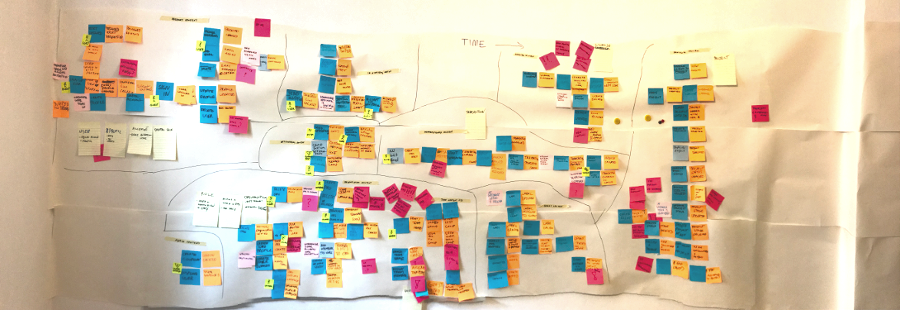
\includegraphics[width=0.75\textwidth]{images/2.1/event-storming}
    \caption{Event Storming Board}
    \label{fig:rlBoard}
\end{figure}

Nachdem initial Domain Events beim \ac{ES} erstellt wurden, soll jedem ein Command vorausgesetzt werden.
Ein Command fungiert hierbei als die Aktion, welche das Event ausgelöst hat.
Dies können Aktionen eines Nutzers oder externen Systems sein.
Während eines Workshops können sogenannte \textit{Hotspots} in Gesprächen entdeckt werden.
Dabei kann es sich um Probleme aber auch Fragen bezüglich des Ablaufs handeln, welche wichtig für die spätere Anwendung werden.

Wie auch das~\ac{DDD} kann Event Storming jederzeit während des Entwicklungsprozesses verwendet werden.
Für die verschiedenen Anwendungsbereiche hat Brandolini mehrere Typen des Event Stormings definiert.
Hierbei bleibt die Methodik an sich die gleiche, allerdings wird das Ziel genauer definiert.\newline
\textbf{Big Picture EventStorming} wird während eines Kick-off Meetings eingesetzt, damit alle Teilnehmer den Inhalt und den Bereich der zur erstellenden Anwendung kennenlernen.
Hierzu ist es nötig, dass alle Interessengruppen vertreten sind, welche innerhalb des Unternehmens existieren und ebenfalls eine Entscheidungsgewalt innehaben.\newline
\textbf{Design Level EventStorming} findet auf einer tieferen Ebene einen Einsatz.
Dabei handelt es sich um das Erstellen möglicher Implementierungen, zum Beispiel, ob Event Sourcing oder andere Techniken aus dem~\ac{DDD} verwendet werden sollen.
Es werden somit Entscheidungen getroffen, welcher in erster Linie die Entwickler betrifft und von diesen am besten zu bewerten ist.\newline
\textbf{Value-Driven EventStorming} bietet einen Einstieg in die Wertstromanalyse (englisch: value-stream mapping).
Anhand einer solchen Analyse ist es möglich den Erhalt von Informationen und der Verarbeitung dieser darzustellen und Probleme zu erkennen.\newline
\textbf{UX-Driven EventStorming} konzentriert sich auf das Erlebnis eines Nutzers/Kunden bei der Benutzung der Anwendung.
Hierbei wird neben der Nutzerfreundlichkeit auch die fehlerfreie Ausführung abgebildet und überprüft.\newline
\textbf{EventStorming as a Retrospective} konzentriert sich darauf einen Ablauf über Domain Events zu definieren und nach
Erweiterungsmöglichkeiten zu suchen, welche Vorteile für die Anwendung bereitstellen können.\newline
\textbf{EventStorming as a Learning Tool} zeigt auch die weiteren Lernchancen innerhalb eines Unternehmens.
Mittels Event Storming ist es somit auch möglich neue Angestellte möglichst schnell auf den aktuellen Stand zu bringen.
Diese Art von Lernchancen ist ebenfalls im~\textbf{Big Picture EventStorming} enthalten.

\subsection{Erweiterung}\label{subsec:erweiterung}
\todo{Hier das vorherige Kapitel abwarten um alle Änderungen/Erweiterungen besser daran fest zu machen.}
\begin{itemize}
    \item Erweiterungen für Wirtschaft (Pages -> daraus generierte Mockups, abgehen von dem "Wir wollen keinen PC benutzen" des ES)
    \item Ideen für die Lehre (Wird in dieser Arbeit nicht näher beleuchtet, da es für den Beleg der Funktionalität nicht mehr möglich ist dies ausreichend in der Bearbeitungszeit zu machen)
    \item ES -> Ablauf von Schritten -> Albert -> Workflow (Arbeitsablauf) beschreibungen -> Mögliche Idee zum besseren Nahebringen von komplexeren Abläufen in Vorlesungen. (Verbildlichung)
\end{itemize}


\section{Technologien}\label{sec:technologien}
Dieses Kapitel gibt einen Überblick über die verwendeten Technologien in der Umsetzung.
Da die Implementierung aus verschiedenen Komponenten besteht, ist dieses Kapitel in drei weitere Unterkapitel aufgeteilt.
Es wird somit getrennt auf die Java Library~\textit{fulibWorkflows}, das Spring Boot Backend des~\textit{fulibWorkflows Web-Editors}
und das zum Editor dazugehörige Frontend, welches mit Angular umgesetzt wurde, eingegangen.

\subsection{fulibWorkflows}\label{subsec:fulibworkflows}
\textit{fulibWorkflows} ist eine Java Library, welche Arbeitsabläufe, im Folgenden "workflows", in \ac{YAML}-Syntax notiert, als Eingabe erhält und daraus
sowohl ein Event Storming Board, im Workflow beschriebene Mockups und Objekt-/ Klassendiagramme generiert.
Welche Form die YAML-Eingabe haben muss und wie die Dateien aussehen und generiert werden, wird in Kapitel~\ref{subsec:workflow-format} erläutert.

\subsubsection{Antlr}\label{subsubsec:antlr}
\ac{Antlr} bietet die Möglichkeit einen Parser über eine eigens geschriebene Grammatik zu generieren.
Die Grammatik muss Links ableitend sein und ist in~\ac{EBNF} definiert.
Der generierte Parser ermöglicht zudem das Aufbauen und Ablaufen eines~\textit{Parse trees}.
Hierdurch ergibt sich die Möglichkeit, während dem Parsen weitere Aktionen durchzuführen, welche den späteren Programmablauf eines Tools unterstützen können.

\begin{listing}[!ht]
    \inputminted{antlr-java}{listings/2.2.1/AntlrExample.g4}
    \caption{Beispiel einer einfachen Grammatik in Antlr}
    \label{listing:grammar-example}
\end{listing}

In Listing~\ref{listing:grammar-example} ist ein Beispiel für eine einfache Grammatik zur Erkennung von mathematischen Gleichungen dargestellt.\cite{antlrOrg}
Hierbei ist es lediglich möglich Zahlen mittels Klammern, Addition, Subtraktion, Multiplikation und Division miteinander zu kombinieren.
Die Länge eines Ausdruckes ist durch den rekursiven Aufbau der Grammatik nicht begrenzt.

\begin{listing}[!ht]
    \begin{minted}{text}
    ((199+2324)*43)/55

    \end{minted}
    \caption{Einfacher mathematischer Ausdruck}
    \label{listing:mathematical-input}
\end{listing}

Die zuvor beschriebene Grammatik kann mittels weiterer Tools auf eine Eingabe geprüft werden.
Eine zulässige Eingabe für die festgelegte Grammatik aus Listing~\ref{listing:grammar-example} ist in Listing~\ref{listing:mathematical-input} dargestellt.
Die Überprüfung auf die Richtigkeit einer Eingabe oder auch der Grammatik kann über Tools bereits vor einer Generierung von Code durchgeführt werden.
Hierzu wurde das Diagramm aus Abbildung~\ref{fig:parse-example} mittels dem Antlr Plugin für IntelliJ generiert.

\begin{figure}[h]
    \centering
    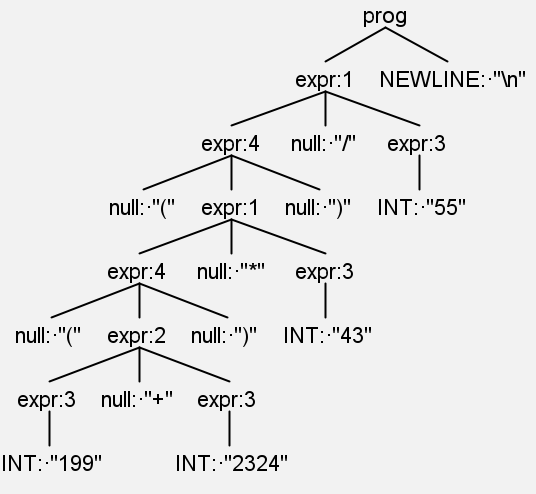
\includegraphics[width=0.3\textwidth]{images/2.2/parseTreeExample}
    \caption{ParseTree für einen mathematischen Ausdruck}
    \label{fig:parse-example}
\end{figure}

Hierbei ist ersichtlich, dass die Wurzel bei der obersten Regel~\textbf{prog} beginnt und alle weiteren Kindknoten durch verschachtelte~\textbf{expr} Regeln kreiert wurden.
Der oberste Teilausdruck ist die Division aus einem komplexeren linken Ausdruck und dem rechten Ausdruck, welcher direkt einer Nummer zugeordnet werden konnte und somit keine weiteren Kindknoten mehr haben kann.
Dies entsteht durch die Unterscheidung bei der Grammatik in Terminale und Nicht-Terminale.
Hierbei werden wie in Listing~\ref{listing:grammar-example} dargestellt Nicht-Terminale Regeln kleingeschrieben und Terminale Regeln werden in Großbuchstaben verfasst.
In der vereinfachten Grammatik sind lediglich ganze Zahlen als Eingabe erlaubt.

Dies sind lediglich die Grundlagen von Antlr, auf die genauere Verwendung des generierten Parsers und Besonderheiten der Grammatik wird in Kapitel~\ref{subsec:antlr-grammatik},
anhand der Implementierung, eingegangen.

\subsubsection{String Template}
\ac{ST} gehört, wie das vorherige \ac{Antlr}, zum~\textit{Antlr Project}.
\ac{Antlr} verwendet ebenfalls \ac{ST}s zur Generierung von formatiertem Text, im Folgenden als \textit{Code} bezeichnet.
Templates (übersetzt: Schablone) ermöglichen es zum Beispiel die feste Syntax einer Programmiersprache mit variablen Werten für
Variablen, Klassen und Methoden zu belegen.
Somit können die generellen Bausteine einer Sprache beliebig gefüllt werden.
Durch diese Funktionalität bieten sich \ac{ST}s sehr gut zur Generierung von Dateien an.
Ursprünglich ist \textit{StringTemplate} eine Java Library, jedoch wurden bereits Portierungen für C\#, Objective-C, JavaScript und Scala erstellt.

Die folgenden Erläuterungen beziehen sich auf die Java Library von \textit{StringTemplate}, da diese in dieser Arbeit verwendet wird.
Die einfachste Möglichkeit für die Verwendung eines String Templates ist in Listing~\ref{listing:simpleTemplate} zu sehen.

\begin{listing}[!ht]
    \inputminted{java}{listings/2.2.1/JavaStringTemplateExample.java}
    \caption{``Hello World!'' - Beispiel mittels StringTemplate}
    \label{listing:simpleTemplate}
\end{listing}

Die Klasse \textit{ST} aus Zeile 3 kann mit einem String initialisiert werden.
In diesem Beispiel wurden als Begrenzer für das zu ersetzende Stück des Textes \textit{<>} verwendet.
Im Anschluss wird dem neuen \textit{ST} Objekt mithilfe der add()-Methode ein bestimmter Wert hinzugefügt.
Der erste Parameter der Methode ist der Bezeichner innerhalb eines Templates, zu beachten ist die Angabe des Bezeichners ohne die Begrenzer.
Der Wert wird als zweiter Parameter übergeben und besitzt in diesem Beispiel den Text \textbf{World}.
Um nun den fertig ersetzten Text aus dem Template und dem übergebenem Wert zu bekommen, muss auf dem \textit{ST} Objekt die Methode render() aufgerufen werden.
Hierbei werden die Platzhalter des Templates durch den zuvor übergebenen Wert ersetzt und als String zurückgegeben.
In Zeile 6 wird nun abschließend der fertige Text auf der Konsole ausgegeben, \texttt{Hello, World!}.
Dieses Beispiel entstammt der offiziellen Webseite von \textit{StringTemplate}.\cite*{stOrg}

Für ein strukturiertes Arbeiten mit vielen Templates bietet \textit{StringTemplate} die Möglichkeit \ac{STG}s zu erstellen.
Hierbei können mehrere Templates in einer Datei beschrieben werden, um aufeinander aufbauende Templates nicht im Code, sondern einer gesonderten Datei zu organisieren.
In diesen Dateien, welche die Dateiendung \textbf{.stg} tragen, können die Begrenzer (eng.: Delimiters) frei gewählt werden.
Dies ist je nach Kontext des Templates nötig, da zum Beispiel die Generierung von HTML-Dateien, welche \textit{<>} als Zeichen zum Abgrenzen von Bereichen verwenden.
Bei der Wahl der Begrenzer sollte somit stets auf die Wahl der Zeichen im Kontext der zu generierenden Sprache geachtet werden.
Zum Parsen einer \ac{STG} wird ein mit Antlr generierter Parser verwendet.\cite*{stgParser}

\begin{listing}[ht]
    \inputminted{c}{listings/2.2.1/Example.stg}
    \caption{Beispiel einer .stg-Datei}
    \label{listing:stgFile}
\end{listing}

Wie zuvor beschrieben ist in Listing~\ref{listing:stgFile} zu erkennen, dass in Zeile 1 die Begrenzer auf~\texttt{\{\}} gesetzt wurden.
Dies hat den Hintergrund, dass in diesem Beispiel ein Text in eine HTML-Datei generiert werden soll.
Hierfür könnten auch die Standardbegrenzer verwendet werden, allerdings müssten dann für Schlüsselwörter wie~\texttt{<span>} die Zeichen < und > mit einem führenden Backslash definiert werden.
Da dies für HTML-Dateien allerdings einen immensen Aufwand bedeutet, macht die Nutzung anderer Begrenzer Sinn.
In Zeile 3 werden für ein~\ac{ST}, sowohl der Name des Templates, als auch Übergabeparameter definiert.
Ein~\ac{ST} wird durch \textit{>>} geschlossen.
Die Begrenzer in Zeile 5 zeigen, dass alles, was sich zwischen Ihnen befindet, einen Übergabeparameter in sich trägt.
Somit ist das Wiederverwenden des Templates und die variable Befüllung gewährleistet.

Um diese Templates nun in einem Java Programm zu verwenden, benötigt es unter anderem die zuvor beschriebenen ST Klasse, sowie
die Klasse \textit{STGroupFile}, welche für die Verwaltung der stg-Datei, als auch deren Templates, benötigt wird.
In Zeile 6 von Listing~\ref{listing:stgJavaFile} ist zu erkennen, dass einem STGroupFile-Objekt bei der Initialisierung eine URL übergeben werden muss.
Diese URL verweist auf die stg-Datei.
Im Anschluss kann, wie in Zeile 8 ersichtlich, über die getInstanceOf()-Methode auf ein bestimmtes Template in der stg-Datei zugegriffen werden.
Hierbei ist es wichtig, keine Fehler bei der Benennung zu machen.
Schließlich ist die weiterführende Verwendung bereits zuvor mittels der ST-Klasse beschrieben worden.

\begin{listing}[!ht]
    \inputminted{java}{listings/2.2.1/JavaSTGExample.java}
    \caption{Nutzung einer STG-Datei in Java}
    \label{listing:stgJavaFile}
\end{listing}

Bei der Ausführung dieses Beispiels wird auf der Konsole der Text aus Listing~\ref{listing:outputSTG} angezeigt.

\begin{listing}[!ht]
    \begin{minted}{html}
<span>
    This test about the university is written in english.
</span>
    \end{minted}
    \caption{STG Ausgabe auf Konsole}
    \label{listing:outputSTG}
\end{listing}

\subsubsection{JSON-Schema}\label{subsubsec:json-schema}
JSON-Schemas sind Schemata, welche den Inhalt einer JSON-/YAML-Datei begrenzen können.
Hierdurch ist es möglich, den Nutzer in seinen Eingaben zu begrenzen und bereits während dem Schreiben einer Datei dabei zu unterstützen sinnvolle Eingaben zu erstellen.
In dieser Arbeit wird lediglich auf die Nutzung der Schema Version 7, die neuste Version, eingegangen, da diese in der Anwendung verwendet wird.

JSON Schemas können Objektstrukturen in beliebiger Tiefe schachteln.
Im folgenden Abschnitt werden die grundlegenden Elemente eines JSON Schemas erläutert.
Weiterführende Funktionalitäten werden anhand der Implementierung in Kapitel~\ref{subsec:schema} näher beleuchtet.

Ein einzelnes Objekt kann zur Verbesserung der späteren Nutzung mit einem Titel und einer kurzen Beschreibung versehen werden.
Diese sind in Listing~\ref{listing:objectSchema} in Zeile 2 und 3 dargestellt.
\textit{title} und \textit{description} dienen lediglich der verbesserten Lesbarkeit für den Entwickler.

\begin{listing}[!ht]
    \inputminted{json}{listings/2.2.1/object.schema.json}
    \caption{Objekt Beispiel eines JSON Schemas}
    \label{listing:objectSchema}
\end{listing}

Einem Element muss stets ein \textit{type}, also ein Typ, zugeordnet werden.
Dies kann entweder ein Objekt, Zeile 4 in Listing~\ref{listing:objectSchema}, oder eine Liste sein.
Einem Objekt können nun \textit{properties} hinzugefügt werden.
Diese besitzen neben einem eindeutigen Bezeichner ebenfalls eine Beschreibung und einen Typen.
Auf dieser Ebene kann der Typ eine Nummer, \textit{integer} in Zeile 8, oder auch ein Text, welches den Typ \textit{string} bekommen würde, sein.
Ist eine der \textit{Properties} ein notwendiges Feld, kann dies mittels des Schlüsselwortes \textit{required} realisiert werden.
Hierbei wird eine Liste an Bezeichnern hinterlegt, welche dem Objekt bereits zugeordnet wurden und somit stets vorhanden sein müssen.
Das Beispiel stammt von der offiziellen JSON Schema Webseite.\cite*{schemaExample}
Sollten einem Objekt keine weiteren properties hinzugefügt werden dürfen, ist dies mit dem Ausdruck aus Listing~\ref{listing:additionalProperties} möglich.

\begin{listing}[!ht]
    \begin{minted}{json}
"additionalProperties": false
    \end{minted}
    \caption{Begrenzung der Properties eines Schemas}
    \label{listing:additionalProperties}
\end{listing}

Wie zuvor bereits beschrieben, kann ein Element auch als Liste deklariert werden.
Dies ist an einem kleinen Beispiel in Listing~\ref{listing:listSchema} dargestellt.
Hierbei ist es möglich die \textit{items} einer Liste genauer zu definieren.
In diesem Beispiel müssen die Elemente einer Liste dem Schema aus dem Beispiel aus Listing~\ref{listing:objectSchema} entsprechen.

Eine JSON-/YAML-Datei, welchem dieses Schema zugrunde liegt, besteht somit aus einer Liste an Produkten.
Durch die Verwendung des \textit{oneOf} Operators in Zeile 6, werden nur Elemente mit dem darunterliegenden Schema akzeptiert.
Bei mehreren Einträgen in der \textit{items} Aufzählung muss immer eines dieser Elemente auf das Objekt in der JSON-/YAML-Datei zutreffen.

\begin{listing}[!ht]
    \inputminted{json}{listings/2.2.1/list.schema.json}
    \caption{Listen Beispiel eines JSON Schemas}
    \label{listing:listSchema}
\end{listing}

Durch ein fest definiertes Schema ist es vielen IDEs, darunter auch IntelliJ und VSCode,
möglich den Entwickler durch Fehlerhervorhebung und Autovervollständigung zu unterstützen.
Hierfür ist es möglich bereits erstellte JSON-Schemas im \textit{SchemaStore} bereitzustellen.
Dies ist eine zentrale Stelle, um JSON-Schemas für IDEs zur Verfügung zu stellen.
Bei dem \textit{SchemaStore} handelt es sich um ein Open-Source-Projekt, bei welchem die Einbringung eines neuen Schemas simpel gestaltet ist.
Es ist möglich ein fertiges Schema fest dort zu hinterlegen, hierdurch muss für jede neue Änderung allerdings ein neuer Betrag erstellt werden.
Dieser bedarf einer Zustimmung einem der Verwalter des \textit{Schema Stores}.
Da dies stets mit einer Verzögerung passiert, ist es möglich eine Verlinkung zu einem Schema zu erstellen.
Somit können Änderungen an einem Schema durchgeführt werden, um diese Änderungen nach dem Hochladen direkt zur Verfügung stellen zu können.
Zum aktuellen Zeitpunkt existieren 439 Schemas, welche durch \textit{SchemaStore.org} für diverse IDEs bereitgestellt werden.\cite*{schemaStore}
Eine Liste aller IDEs, welche diesen Support mittels \textit{schemastore} unterstützen sind unter folgendem
Link zu finden: \url{https://www.schemastore.org/json/#editors}

\subsubsection{fulibTools}
FulibTools ist Teil der Fujaba Tool Suite, auch das in dieser Arbeit erstellte fulibWorkflows ist ein Teil der Fujaba Tool Suite.
Fulib bildet die Grundlage für fulibTools, wobei fulibTools erweiterte Möglichkeiten für die Nutzung von fulib bereitstellt.
Fulib ist ein Codegenerator, welcher mittels einer~\ac{DSL}, Modelle als Diagramme darstellen kann.\cite*{fulib}
Dies begrenzt sich nicht nur auf Klassenmodelle, sondern ist auch für Objektmodelle einsetzbar.
FulibTools ist eine Erweiterung, da die Generierung der Diagramme auch abseits der eben erwähnten DSL funktioniert.\cite*{fulibTools}
Hierdurch bietet sich die Möglichkeit Objektmodelle über ein spezielles YAML-Format oder ein Java Objektmodell zur Laufzeit zu generieren.
Gleiches gilt für Klassenmodelle.
Die Verwendung von FulibTools ist somit für diese Arbeit eine bessere Wahl, als \textit{Graphviz}, eine Bibliothek zur Generierung von Diagrammen, direkt zu verwenden.
Dies ist der Fall, da FulibTools bereits die Arbeit der Verarbeitung einer Eingabe übernimmt und hierdurch leichter für ein weiteres Tool der Fujaba Tool Suite zu verwenden ist.


\subsection{Frontend des Web-Editors}\label{subsec:fulibworkflows-web-editor}
Der Web-Editor für fulibWorkflows besteht aus einem Frontend und einem Backend.
Dieses Kapitel beschäftigt sich mit den Technologien, welche für das Frontend verwendet werden.
Hierbei wurde die Entscheidung über die verwendeten Technologien für die Integration des Editors in die Webseite \url{fulib.org} getroffen.
Auf diese Integration wird in Kapitel~\ref{ch:fazit} näher eingegangen.

\subsubsection{Angular}
Die Grundlage für das Frontend ist Angular.
Angular ist ein Framework für das Designen von Applikationen und gleichzeitig eine Entwicklungsplattform\cite*{angular}.
Für Entwickler ist das Angular Command-Line-Interface ein wichtiger Bestandteil bei der Entwicklung mit Angular.
Neben der Generierung einer neuen Anwendung können ebenfalls neue Komponenten, Services und Module generiert werden.
Die \textit{Komponenten} dienen der Strukturierung einer Anwendung und enthalten verschiedene Abschnitte ebendieser.
Hierbei besteht ein großer Vorteil darin, Komponenten modular zu gestalten.
Dies bedeutet, dass Komponenten so entwickelt werden, dass diese in der Anwendung wiederverwendet werden können, sollte dies möglich sein.
Eine Komponente besteht aus drei einzelnen Bereichen:

\begin{enumerate}
    \item Der Logik, welche in Typescript verfasst wird.
    \item Einem Template, welches eine HTML-Datei ist.
    \item Styles, welche im Template eingebunden werden können, um die Oberfläche grafisch zu verändern.
\end{enumerate}

Im Template werden neben den Styles auch Bestandteile des Code-Segments verwendet, um Daten dynamisch anzeigen zu können.
Ein neu generiertes Angular Projekt bietet allerdings nur die Grundlage einer Anwendung.
Um weitere Funktionalitäten in der Anwendung verwenden zu können, können sogenannte Package Manager wie \textit{npm} oder \textit{yarn}
verwendet werden, um neue Bibliotheken einzubinden.

Auf weitere Erklärungen wird an dieser Stelle verzichtet, da Angular in Gänze zu erklären den Rahmen dieser Arbeit überschreiten würde.
In Kapitel~\ref{sec:editor-frontend} wird auf weitere Funktionen genauer eingegangen und diese anhand der Implementierung erklärt.
Folgend werden Bibliotheken erläutert, welche die wichtigsten Bestandteile der Anwendung ermöglichen.

\subsubsection{Bootstrap}
Um eine Oberfläche zu gestalten, welche einheitlich mit der von \textit{fulib.org} sein soll, wurde Bootstrap zum
Stylen der Oberflächenelemente verwendet.
Bootstrap bietet diverse Komponenten wie Eingabefelder, Buttons, Menüs, Pop-Ups und viele weitere.
Neben den Styles enthalten diese auch zusätzliche Funktionen, welche im Kontext der Komponente sinnvoll sind.
Dabei bleibt es weiterhin abänderbar, um dem Entwickler mehr Freiheiten zur Gestaltung einer Oberfläche zu geben.
Weiterhin ermöglicht es Bootstrap das Layout, also die Anordnung, von Komponenten auf einer Seite festzulegen.
Dies beginnt bei der Größe einer Komponente bis hin zu der Anordnung in der Horizontalen und Vertikalen\cite*{bs}.

Zusätzlich zu Bootstrap wurden Bootstrap Icons verwendet, um die Oberfläche mit Symbolen zu versehen.
Hierbei handelt es sich um eine Sammlung von rund über 1500 Icons, welche frei verwendbar sind\cite*{bsIcons}.

\subsubsection{CodeMirror}
CodeMirror ist ein Texteditor, welcher in JavaScript geschrieben wurde und somit in Web-Anwendungen verwendet werden kann.
Es gibt zahlreiche Optionen, um CodeMirror an die Bedingungen der zu bauenden Anwendung anzupassen.
Neben zahlreichen Programmiersprachen, welche durch das Hervorheben von Schlüsselwörtern und der Überprüfung der Syntax emuliert werden können,
ist es möglich CodeMirror zu einer eigenen, individualisierten IDE zu konfigurieren.
Erweiterungen für einen CodeMirror sind die sogenannten Add-Ons.
Hierbei gibt es neben vielen bereits vorhandenen Erweiterungen auch die Möglichkeit eigene Add-Ons zu erstellen.
Hierzu zählt unter anderem das zuvor erwähnte farbliche Hervorheben von Schlüsselwörtern, auch Highlighting genannt, wie auch die
Überprüfung des Codes auf die Syntax der eingestellten Programmiersprache\cite*{cm}.

Für eine einfache Einbindung in ein Angular-Projekt existieren bereits mehrere Bibliotheken, welche eine CodeMirror-Komponente bereitstellen.
Bei dieser Komponente können nicht nur Optionen übergeben, sondern auch der Inhalt eines CodeMirrors, also den geschriebenen Code, aus der Komponente
extrahiert werden.
In dieser Arbeit wird hierzu ngx-codemirror von Scott Cooper verwendet\cite*{ngxcm}.


\subsection{fulibWorkflows Web-Editor Backend}\label{subsec:backend}
Das folgende Kapitel beschäftigt sich mit dem zweiten Bestandteil des Web-Editors, das Backend.
Vom Frontend wird eine YAML-Beschreibung ans Backend geschickt, in diesem wird dies als Eingabe für fulibWorkflows verwendet.
Da fulibWorkflows eine Java-Bibliothek ist, benötigt es ein Backend, welches auf Java basiert.

\subsubsection{Spring Boot}
Mittels \textit{Spring Boot} ist es möglich schnell und ohne zusätzliche Konfiguration eine auf \textit{Spring} basierende Applikation zu erstellen.\cite*{springBoot}
Spring ist ein Framework, welches sich als Ziel gesetzt hat Java Programmierung zu vereinfachen und zu verschnellern, allerdings keine Einbußen
bei Geschwindigkeit, Komplexität und Produktivität zu machen.\cite*{spring}
In diesem Kapitel wird sich mit der Erstellung eines Rest-Services befasst.
Ein Rest-Service stellt Endpunkte bereit, welche über REST angesprochen werden können.
Diese eignen sich zur Nutzung als simples Backend.

\begin{figure}[h]
    \centering
    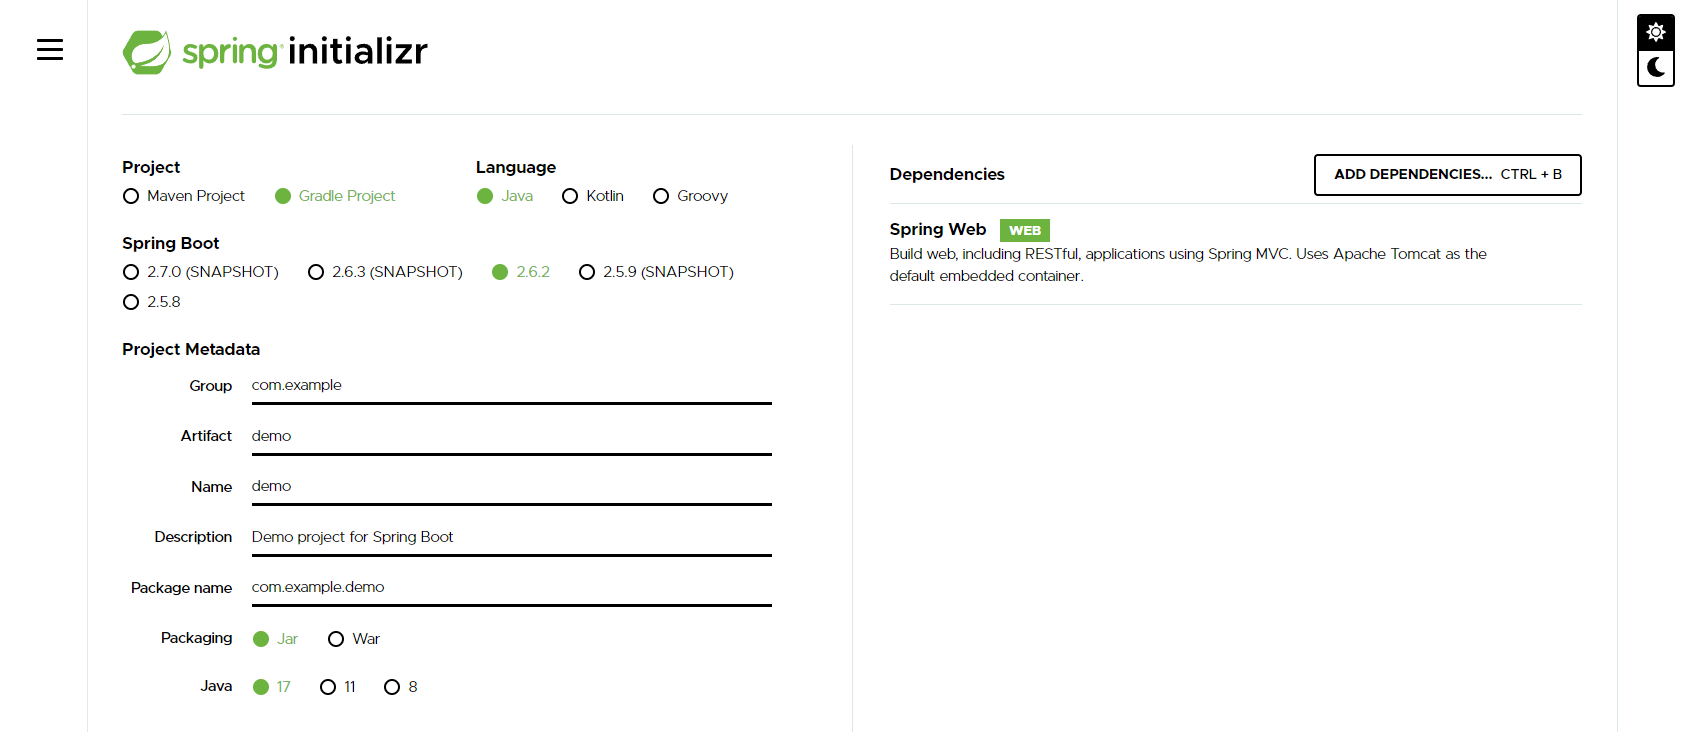
\includegraphics[width=1.0\textwidth]{images/2.2/spring-init}
    \caption{Spring Initalizr für eine Web Anwendung}
    \label{fig:spring-init}
\end{figure}


Das Anlegen eines Spring Boot Projektes kann durch den \textit{Spring Initializr} erledigt werden.\cite*{sbinit}
In Abbildung~\ref{fig:spring-init} ist dieser zu sehen.
Hierbei können diverse Einstellungen getätigt werden, um das zu generierende Projekt an die Anforderungen des Generierenden anzupassen.
Die Abbildung zeigt die getätigten Einstellungen, um ein Gradle Projekt mit Java, Version 17, als Programmiersprache zu generieren.
Ebenfalls kann die Version von Spring Boot eingestellt werden.
Zusätzliche Dependencies können im rechten Bereich des \textit{Spring Initializrs} hinzugefügt werden.
In diesem Fall wurde \textbf{Spring Web} ausgewählt, wodurch die wichtigsten Dependencies für eine REST Applikation bereits enthalten sind.

Das aus den vorherigen Einstellungen beschriebene Projekt ist bereits ein fertiges Backend, welches direkt ausgeführt werden kann.
Durch sogenannte Annotations, welche mit einem @ gekennzeichnet werden, ist es möglich weitere Endpunkte für das Backend zu definieren.
Auf die genaueren Funktionen, welche mittels Annotations implementiert werden können, wird in Kapitel~\ref{sec:editor-backend} eingegangen, anhand von Beispielen der Implementierung.



\subsection{Deployment}\label{subsec:deployment}
\todo{this}
Ein Web Editor will natürlich für alle erreichbar sein.
Und fulibWorkflows muss auch irgendwo bereitgestellt werden, damit es das Backend und alle anderen
interessierten benutzen können.

\subsubsection{MavenCentral}\label{subsubsec:mavencentral}
\todo{this}
MavenCentral ein wirklicher Hussarones was das publishen angeht.
Glücklicherweise ist fulibWorkflows Teil der Fujaba Tool Suite, wodurch die benötigten
Zugriffsrechte bereits vorhanden und andere Libraries bereits gepublished wurden.
Hierdurch war es recht schnell möglich mit dem zuvor erworbenem Wissen fulibWorkflows
zu publishen.

\subsubsection{Heroku}\label{subsubsec:heroku}
\todo{this}
Der Web-Editor soll immer erreichbar sein.
Dies ist durch Heroku nur bedingt möglich.
Heroku bietet allerlei Möglichkeiten verschiedenste Anwendungen bereitzustellen.
Auch mit einem kostenlosen Plan ist es ohne Probleme möglich solch kleine Anwendungen bereitzustellen.

FE Deployment war easy, auch wenn ich erstmal wieder in eins meiner früheren Projekte gucken musste.
BE Deployment war kniffliger, doch man ist nie der erste der eine Spring Boot application
auf Heroku deployen will.
Daher Tutorial reingefahren und ab ging der gebutterte Lachs.


